\documentclass[12pt]{article}

\usepackage[utf8]{inputenc}
\usepackage{latexsym,amsfonts,amssymb,amsthm,amsmath,setspace,graphicx}

\setlength{\parindent}{0in}
\setlength{\oddsidemargin}{0in}
\setlength{\textwidth}{6.5in}
\setlength{\textheight}{8.8in}
\setlength{\topmargin}{0in}
\setlength{\headheight}{18pt}



\title{ Sheet 3 }
\author{Ivakhnenko Bohdana, König Marvin Anton, Mayers Christophe}

\begin{document}

\maketitle

\vspace{0.5in}



\subsection*{Exercise 1}
\begin{itemize}

\item[Task 1.] 
\[
R_{emp}(f|D) \overset{a. s.}{\longrightarrow} R(f)
\]
$R_{emp}(f|D) = \frac{1}{N} \sum_{i=1}^NL(y_i, f(x_i))$\\\\
$(x_i,y_i)\sim p(x,y)$ is i.i.d, so\\\\
$\frac{1}{N}\sum_{i=1}^NL(y_i, f(x_i))\overset{LLN}{\longrightarrow}E[L(y_i, f(x_i))]$ ,\\\\  $L(\overset{\sim}{f}(x) = y, f(x)) \longrightarrow L(y, f(x))$ \hspace{0.5cm}for $N \longrightarrow \infty \hspace{0.5cm} \Longrightarrow$ \\\\
$R_{emp}(f|D) = \frac{1}{N} \sum_{i=1}^NL(y_i, f(x_i)) \overset{LLN}{\longrightarrow} E[L(y_i, f(x_i))] = R(f) \hspace{0.5cm} $for $ N \longrightarrow \infty $
\\\\
\item[Task 2.] 
\begin{itemize}
\item[(a)] Due to the high variance $f_2$ has, it learns the fluctuations of the data set and reacts completely differently when new data are included.\\
On the other side, $f_1$s high bias hinders the model to archive good predictions but is robuster and therefore less susceptible to overfitting.\\

\item[(b)]
Figure 1.
\begin{figure}
    \centering
    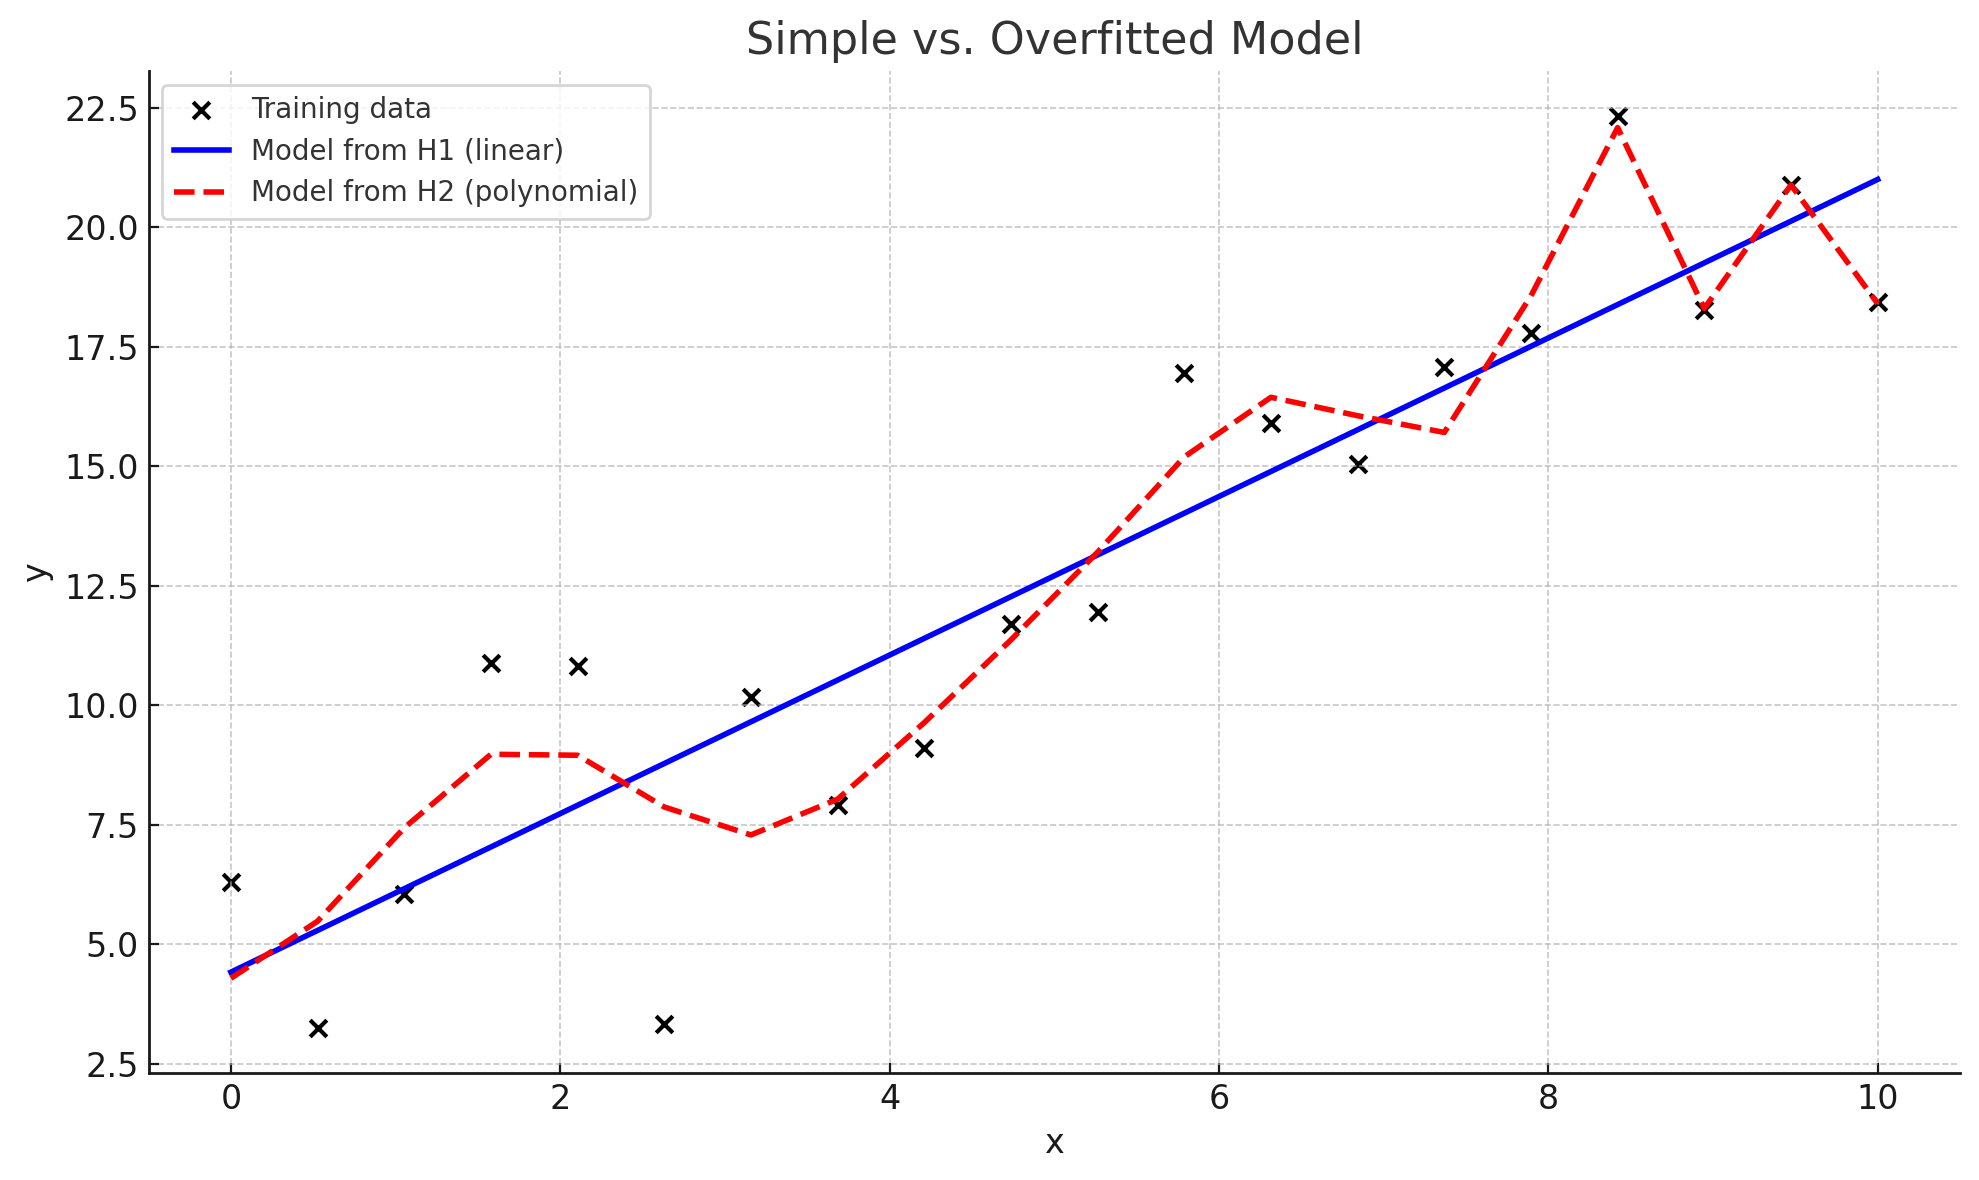
\includegraphics[width=1\linewidth]{image.png}
    \caption{linear Trend with noise}
\end{figure}

\item[(c)] 


\end{itemize}
\end{itemize}

\end{document}
